\section{Error Analysis}
\label{sec:errors}

% Budget: about 0.8 column-pages plus one figure. Rubric: 5 pts, the largest report item.
% "Real failure cases shown, patterns identified, explanations proposed."
% Sources: Section 8.3b (fig11b_error_corrected, fig11c_error_persistent,
% table_error_pairs.csv, table_error_by_class.csv, table_error_by_driver.csv),
% Section 8.3 (fig11_gradcam), Section 8.1 (fig09 confusion matrices, fig08 per-class F1).
% Structure:
%   1. Overall error rate of the final model and the top confusion pairs with counts.
%   2. A figure of real failure frames with Grad-CAM (persistent mistakes, plus 1 or 2
%      corrected ones). Check data use rules before showing frames.
%   3. Name each pattern and give a proposed cause (for example c0 vs. c9 differ only by a
%      small head turn, c8 shares the raised hand with the phone classes).
%   4. Per-driver concentration (the worst drivers) and a proposed cause, marked as a
%      hypothesis unless checked.
%   5. Where the full model helps and where it hurts the baseline (frames fixed vs. broken).
% The paragraphs below are the earlier draft from the first model. Replace the numbers with
% the final model's numbers, and replace the figure with fig09 or fig15.

Error analysis included metrics not previously shown for the model to help better determine accuracy, bias, as well as allow us to be able to determine the best modifications for finetuning.
New statistics included: entropy loss, F1 precision, and total accuracy. These were accomplished by using sklearn metrics to be computed after and during the model.

Originally, the model did not fair the best with an accuracy of 51.8\%.
Recall was the highest with the driver operating the radio at 0.91, and steadily declined from mid 0.6 in makeup, texing, and reaching behind range down to 0.16 when talking to the passenger.
Based on how similar some of the poses are such as texting and using the phone, the recall is a significantly higher due to the clusters it creates by similarity.

The largest issue that can be denoted from this data is the inability to generalize new drivers.
Not only is this denoted in the accuracy, but the high cross entropy.

\begin{figure}[t]
  \centering
    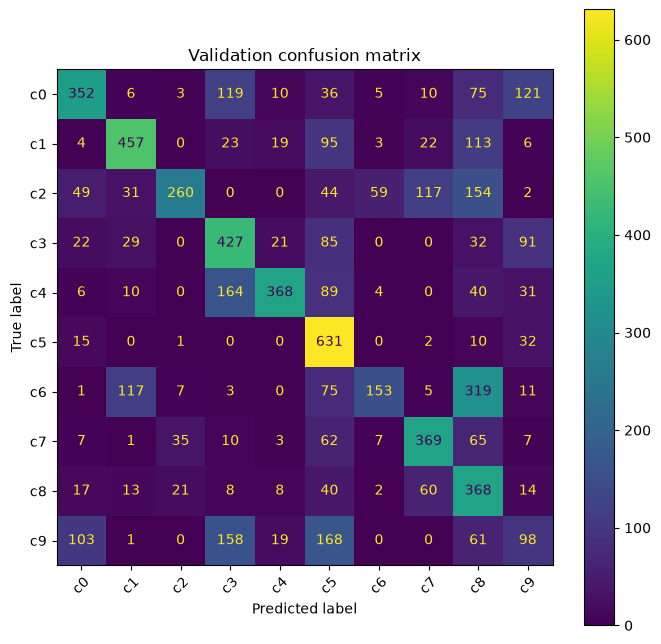
\includegraphics[width=\linewidth]{figures/Val_Conf_Matrix.png}
    \caption{Original confusion matrix after training.}
    \label{ffig:confmat}
  \hfill
\end{figure}

\TODO{Failure-case figure with Grad-CAM, named patterns, and proposed causes.}
